\section{Auswertung}
\label{sec:auswertung}
\subsection{Invariante Masse der B-Mesonen in simulierten Daten}

Zu Beginn werden die \texttt{\.root}-Dateien der simulierten Daten eingelesen und die Features betrachtet.
Das Ziel im ersten Teil ist, die invariante Masse der B-Mesonen zu bestimmen. Da dies nicht direkt funktioniert, muss dies \"uber die Tochterteilchen getan werden.
Betrachten wird ausschie\ss lich der Zerfall
\begin{equation}
  B^{\pm} \to \symup{K}^{\pm} \symup{K}^{+} \symup{K}^{-}\,.
\end{equation}
Um die invariante Masse zu bestimmen wird die Beziehung aus der speziellen Relativit\"atstheorie
\begin{equation}
  \symup{E}^2 = \symup{p}^2 + \symup{m}^2\,,
  \label{eqn:relativityEQ}
\end{equation}
verwendet, welche Energie, Masse und Impuls verkn\"upft.

Aus den Daten werden die Dreierimpulse der Tochterteilchen entnommen.
Diese werden zunächst in einem Diagramm dargestellt um diese zu überprüfen.

\begin{figure}[!htb]
  \centering
  \minipage[c]{0.32\textwidth}
    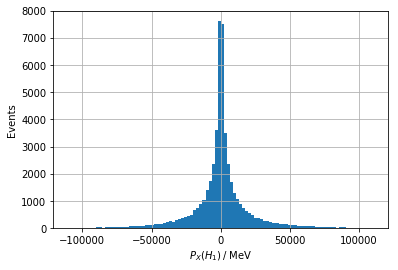
\includegraphics[width=\linewidth]{plots/sim_px_kaon1.png}
    \label{fig:px}
  \endminipage\hfill
  \minipage[c]{0.32\textwidth}
    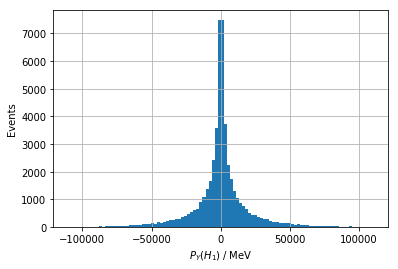
\includegraphics[width=\linewidth]{plots/sim_py_kaon1.png}
    \label{fig:py}
  \endminipage\hfill
  \minipage[c]{0.32\textwidth}
    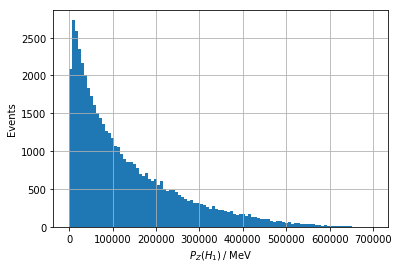
\includegraphics[width=\linewidth]{plots/sim_pz_kaon1.png}
    \label{fig:pz}
  \endminipage
  \caption{Die Impulse in x, y und z Richtung von Kaon1.}
  \label{fig:momenta}
\end{figure}

Es ist in Abbildung \ref{fig:momenta} zu erkennen, dass die Teilchen stark in z-Richtung geboostet sind, was auch zu erwarten ist bei B-Mesonen.

Um die invariante Masse zu berechnen, wird zun\"achst die Energie der B-Mesonen bestimmt, mit 
\begin{equation}
  \symup{E}(B^{\pm}) =
  \sqrt{\left(\sum_{i = 1}^{3} \vec{\symup{p}}_i\right)^2 + \left(\sum_{i = 1}^{3} \symup{m}_i\right)^2} \, .
\end{equation}

F\"ur die Massen wird die Massenhypothese der Kaonen eingesetzt, da dies der interessante Endzustand ist.

Mit der berechneten Energie kann durch umstellen von Gleichung \eqref{eqn:relativityEQ} auf den Impuls und damit auch auf das Betragsquadrat der B-Mesonen geschlossen werden.

In Abbildung \ref{fig:invMassB} liegt der Massenpeak bei etwa $\SI{5279.2}{\mega\electronvolt}$, was sehr eng an dem Wert des PDG (siehe Tabelle \ref{tab:PDGMassen}) liegt.
%Hier müssen wir noch eine Quelle zur PDG Masse einfügen
Dieser Peak ist so scharf, da es sich hier im simulierte Daten handelt. In Wirklichkeit sollte der Peak breiter gefächert sein.

\begin{figure}[!htb]
  \centering
  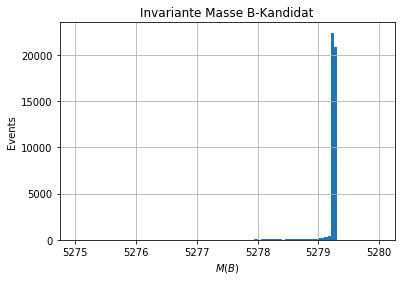
\includegraphics[width=0.8\textwidth]{plots/sim_inv_masse_B.png}
  \caption{Invariante B Masse in den simulierten Daten.}
  \label{fig:invMassB}
\end{figure}

\subsection{Invariante Masse der B-Mesonen in echten Daten}
Als n\"achstes wird die invariante Masse der echten B-Mesonen rekonstruiert.
Hierzu wird zun\"achst eine Vorselektion durchgef\"uhrt um den oben genannten Endzustand zu verwenden.
%Dazu verwenden die folgenden Schnitte.
%\begin{enumerate}
%  \item \texttt{H1\_isMuon} == False
%  \item \texttt{H1\_ProbPi} < 0.5
%  \item \texttt{H1\_ProbK} > 0.5
%\end{enumerate}
Dazu werden die folgenden Schnitte
\begin{enumerate}
  \item \texttt{H1\_isMuon} == False
  \item \texttt{H1\_ProbPi} < 0.5
  \item \texttt{H1\_ProbK} > 0.5
\end{enumerate}
verwendet.

Diese Schnitte werden analog auch f\"ur Tochterteilchen 2 und 3 angewandt.
Dabei bezeichnet der Schnitt $\texttt{H1\_isMuon}$ ob das besagte Teilchen als Myon identifiziert wurde, der Schnitt $\texttt{H1\_ProbPi}$ wie hoch die berechnete Wahrscheinlichkeit ist, dass das Teilchen ein Pion ist und der Schnitt $\texttt{H1\_ProbK}$ wie hoch die berechnete Wahrscheinlichkeit ist, dass das Teilchen ein Kaon ist.
Auf den verwendeten Datensatz sind schon einige Schnitte angewandt worden, diese sind in Tabelle \ref{tab:cuts} im Anhang zu finden.
Die Verteilungen der Wahrscheinlichkeiten ob ein Endzustandsteilchen ein Kaon oder Pion ist werden geplottet um die Schnitte auf \texttt{H1\_ProbK} und \texttt{H1\_ProbPi} sch\"arfer zu machen falls nötig.
Dies hat zur Folge, dass sehr viel Statistik im Signal verloren geht und noch ziemlich viel Hintergrund vorhanden ist. Deswegen werden die Schnitte wie oben belassen.
Die Wahrscheinlichkeitsverteilungen mit unserem hypothetischen Schnitt ist in Abbildung \ref{fig:probCuts} zusehen.

\begin{figure}[!htb]
  \centering
  \minipage[c]{0.48\textwidth}
    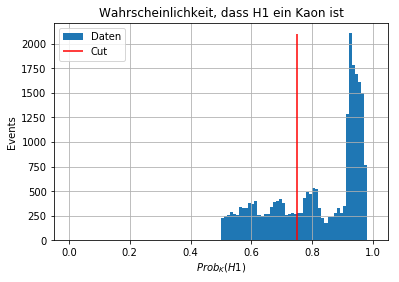
\includegraphics[width=\linewidth]{plots/probability_kaon1.png}
    \label{fig:probK}
  \endminipage\hfill
  \minipage[c]{0.48\textwidth}
    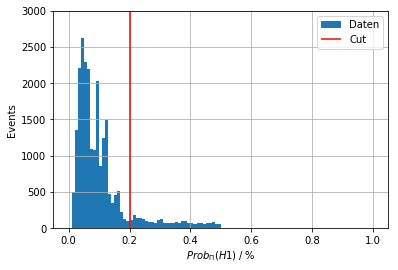
\includegraphics[width=\linewidth]{plots/probability_pion1.png}
    \label{fig:probPi}
  \endminipage
  \caption{Wahrscheinlichkeitsverteilungen f\"ur Kaon und Pion.}
  \label{fig:probCuts}
\end{figure}

Anschlie\ss end wird, wie schon bei den simulierten Daten, die invariante Masse der B-Mesonen berechnet. Diese ist in Abbildung \ref{fig:realBMass} dargestellt.
Analog zu dem Massenplot der simulierten Daten findet sich ein recht scharfer Peak in einem Bereich um die Tats\"achliche B-Meson Masse wieder. Darunter liegt ein exponentiell abfallender Untergrund, welcher in einem Bereich von $\SI{5050}{\mega\electronvolt}$ bis $\SI{5200}{\mega\electronvolt}$ recht prominent ist.

\begin{figure}[htb]
  \centering
  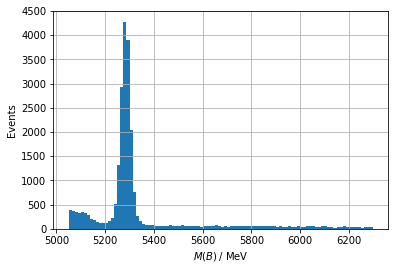
\includegraphics[width=0.8\textwidth]{plots/real_data_inv_masse_B.png}
  \caption{Invariante B Masse in den echten Daten.}
  \label{fig:realBMass}
\end{figure}

\newpage

\subsection{globale CP-Asymmetrie}
\label{sec:globCP}

Um den Materie-Antimaterie Unterschied sichtbar zu machen, m\"ussen $B^{-}$ von den $B^{+}$-Mesonen separiert werden.
Hierzu wird die Ladungen der Tochterteilchen multipliziert.
Ist das Produkt $+1$,wird das Ereignis zu den $B^{-}$ gez\"ahlt, andernfalls zu den $B^{+}$.
Das bedeutet der Asymmetriefaktor berechnet sich gem\"a\ss
\begin{equation}
  \symup{A} = \frac{N^{+} - N^{-}}{N^{+} + N^{-}} = 0.\overline{037} \, .
  \label{eqn:globCP}
\end{equation}

Daraus berechnet sich die statistische Unsicherheit und die Signifikanz mittels
\begin{align}
  \label{eqn:sigmaCP}
  \sigma_A &= \sqrt{\frac{1 - A^2}{N^{+} + N^{-}} } \approx 0.006 \\
  \label{eqn:signifikanzCP}
  \text{Signifikanz} &= \frac{\symup{A}}{\sigma_A} \approx 5.729 \, .
\end{align}

Ohne Ber\"ucksichtigung der systematischen Unsicherheiten gilt dies als Entdeckung der CP-Asymmetrie.
Da es jedoch eine Produktionsasymmetrie von Materie zu Antimaterie von circa $\SI{1}{\percent}$ gibt, wird dies f\"ur die gesamte Unsicherheit mit berechnet. 
Daraus ergibt sich eine Signifikanz von: 
\begin{equation}
  \text{Sig}_{ges} = \frac{\symup{A}}{\sqrt{\sigma_A^2 + 0.01^2}} \approx 3.11 \, .
\end{equation}

Da dieser Wert kleiner als 5$\sigma$ und gr\"o\ss er als 3$\sigma$ ist, gilt die berechnte CP-Asymmetrie nur als Hinweis darauf.

\subsection{Zweik\"orper-Resonanzen f\"ur simulierte Daten}
\label{sec:resosim}
Naiv betrachtet ist der B-Meson Zerfall in drei Kaonen ein Dreik\"orperzerfall, doch es kann auch passieren, dass zun\"achst eine neutral geladene Zwischenresonanz erzeugt wird, welche wiederum in zwei Kaonen zerf\"allt.
Um diese Zwischenresonanzen herauszufiltern werden Dalitz Plots verwendet, da diese Resonanzen als B\"ander sichtbar machen und so leicht identifiziert werden k\"onnen.

Die Kinematik eines Dreik\"orperzerfalls wird eindeutig durch zwei unabh\"angige Variablen ausgedr\"uckt. Hierbei wird die invariante Masse von jeweils zwei der drei Endzustandsteilchen verwendet.
Das bedeutet es gibt drei m\"ogliche Kombinationen:
$M_{1,2}$, $M_{2,3}$, $M_{1,3}$.
Bevor jedoch zwei der Kombinatione ausgew\"ahlt werden k\"onnen, muss die Ladung jedes Tochterteilchens identifiziert worden sein.
Denn die Resonanz muss neutral geladen sein. da aber zwei der drei Teilchen die selbe Ladung besitzen, beispielsweise Teilchen 1 und Teilchen 2, darf $M_{1,2}$ nicht als Variable verwendet werden.
Eine doppelt geladene Resonanz ist au\ss erdem f\"ur Mesonen verboten, da diese immer aus einem Teilchen und einem Antiteilchen bestehen.

In Abbildung \ref{fig:m12} und \ref{fig:m13} sind die Resonanzen f\"ur die Kombinationen $M_{1,2}$ und $M_{1,3}$ dargestellt.

\begin{figure}[htb]
  \centering
  \minipage[c]{0.48\textwidth}
    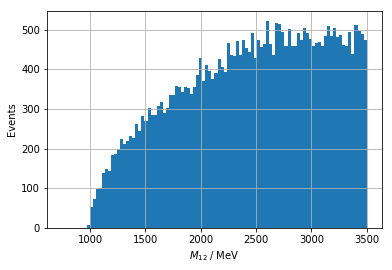
\includegraphics[width=\linewidth]{plots/sim_twobody_resonance_m12.png}
    \caption{Ungeladene Resonanz $M_{1,2}$.\label{fig:m12}}
  \endminipage\hfill
  \minipage[c]{0.48\textwidth}
    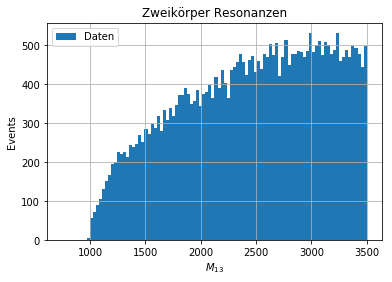
\includegraphics[width=\linewidth]{plots/sim_twobody_resonance_m13.png}
    \caption{Ungeladene Resonanz $M_{1,3}$.\label{fig:m13}}
  \endminipage
  \label{fig:resonances}
\end{figure}
Zu sehen ist hier ein kontinuierliches Spektrum mit ansteigender Anzahl der Events zu h\"oheren Massen f\"ur beide Diagramme.
%Die minimale Masse ist hier die doppelte Kaon Masse und die Obergrenze wird hier bei $\SI{3.5}{\giga\electronvolt}$ gew\"ahlt, da uns h\"oherliegende Resonanzen einerseits nicht interessieren und andererseits irrelevant f\"ur diese Analyse sind, da das B-Meson welches hier untersucht wird selbst nur eine Masse von $\SI{5279.32}{\mega\electronvolt}$ besitzt und aus den Diagrammen nur Charme-Resonanzen hervorkommen sollen.
Die minimale Masse ist hier die doppelte Kaon Masse und die Obergrenze wird bei $\SI{3.5}{\giga\electronvolt}$ gew\"ahlt, da h\"oherliegende Resonanzen einerseits irrelevant f\"ur diese Analyse sind, da das B-Meson welches hier untersucht wird selbst nur eine Masse von $\SI{5279.32}{\mega\electronvolt}$ besitzt und aus den Diagrammen nur Charme-Resonanzen hervorkommen sollen und uns daher andererseits nicht interessieren.

Die quadrierten Massen ergeben aufgetragen gegeneinander den Dalitz Plot, welcher in Abbildung \ref{fig:dalitzSim} zusehen ist.

\begin{figure}[htb]
  \centering
  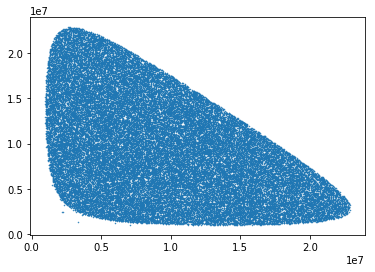
\includegraphics[width=0.8\textwidth]{plots/sim_dalitz_plot_m12_m13.png}
  \caption{Dalitz Plot f\"ur simulierte Daten.}
  \label{fig:dalitzSim}
\end{figure}

Der Dalitz Plot ist kontinuierlich mit Datenpunkten ausgef\"ullt und es sind keine B\"ander erkennbar. Demnach sind in den simulierten Daten keine Resonanzen enthalten.
%Was irgendwo auch erwartbar ist?

\subsection{Zweikörper-Resonanzen für echte Daten}

Wie im vorherigen Abschnitt \ref{sec:resosim} dargestellt lasssen sich über den sogenannten Dalitz Plot etwaige Zwischenresonanzen erkennen.
Dies wird nun für echte Daten analog wiederholt.
Um lediglich Events in der Region der B-Massenresonanz zu berücksichtigen und den Untergrund zu reduzieren wird ein Schnitt auf die B-Masse im Bereich von $\SI{5200}{\mega\electronvolt} < B_M < \SI{5400}{\mega\electronvolt}$ angewandt.
Auch für die echten Daten werden die Größen $M_{1,2}$ und $M_{1,3}$ verwendet.
Dies ist in den Abbildung \ref{fig:rm12} und \ref{fig:rm13} dargestellt.

\begin{figure}
  \centering
  \minipage[c]{0.48\textwidth}%Minipage???
    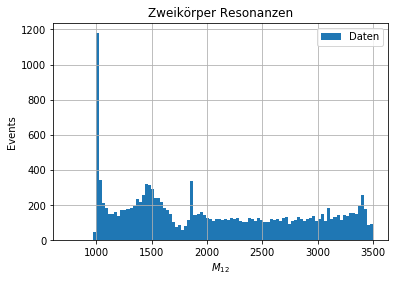
\includegraphics[width=\linewidth]{plots/real_data_twobody_resonance_m12.png}
    \caption{Ungeladene Resonanz $M_{1,2}$.
    \label{fig:rm12}}
  \endminipage\hfill
  \minipage[c]{0.48\textwidth}
    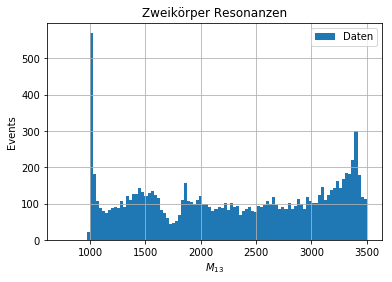
\includegraphics[width=\linewidth]{plots/real_data_twobody_resonance_m13.png}
    \caption{Ungeladene Resonanz $M_{1,3}$.
    \label{fig:rm13}}
  \endminipage
  \label{fig:real_resonances}
\end{figure}

Der Dalitz Plot wird analog zu den simulierten Daten aus den Massenquadraten gebildet.
Dies ist in Abbildung \ref{fig:dalitzReal} zu sehen.
Auffällig sind hier die deutlichen Bänder.
Diese stellen die erwähnten Zwischenresonanzen dar.
Da diese das Ergebnis verfälschen müssen diese im nächsten Schritt entfernt werden.
Um die Resonanzen deutlich sichtbarer zu machen werden die Dalitz Variablen sortiert.
Wie in Abbildung \ref{fig:rm12} und \ref{fig:rm13} zu sehen, weisen die Resonanzen $R_1^0$ und $R_3^0$ dieselbe Verteilung auf.
Dies liegt daran, dass diese aus den gleichen Teilchen $K^+K^-$ zusammengesetzt sind.
Dafür werden die Massen der Resonanzen in $R_\text{Low}^0$ und $R_\text{High}^0$ sortiert.
Also das Kaonpaar mit höherer Masse des Dublets aus $R_1^0$ und $R_3^0$ wird in $R_\text{High}^0$ und das mit niedrigerer Masse wird in $R_\text{Low}^0$ einsortiert.
Werden $R_\text{Low}^0$ und $R_\text{High}^0$ nun als Dalitz Variablen verwendet, wird der vorherige Dalitz Plot nun in einem komprimierteren kinetischen Bereich umgeklappt.
Dies erhöht die Ereignisdichte deutlich und verdeutlicht die Resonanzstrukturen.
Dieser Plot ist in Abbildung \ref{fig:klappeDalitz} dargestellt.

\begin{figure}
  \centering
  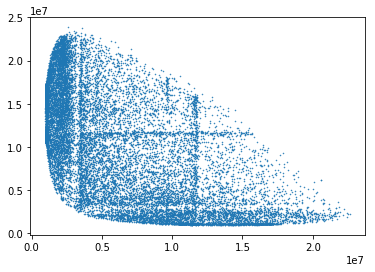
\includegraphics[width=0.8\textwidth]{plots/real_data_dalitz_plot.png}
  \caption{Dalitz Plot für echte Daten.}
  \label{fig:dalitzReal}
\end{figure}

\begin{figure}
  \centering
  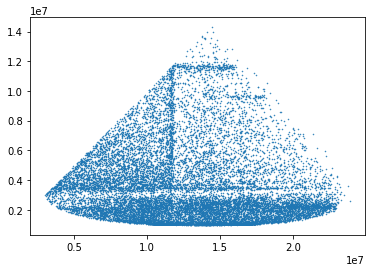
\includegraphics[width=0.8\textwidth]{plots/real_data_sorted_dalitz.png}
  \caption{Umgeklappter Dalitz Plot für echte Daten.}
  \label{fig:klappeDalitz}
\end{figure}

Die Methode, die in Abschnitt \ref{sec:globCP} beschrieben wurde um die CP-Asymmetrie zu untersuchen, ist darauf ausgelegt, dass es sich um charmfreie B-Zerfälle handelt.
Für die simulierten Daten konnte durch den Dalitz Plot in Abbildung \ref{fig:dalitzSim} gezeigt werden, dass keine Charm-Zwischenresonanzen vorhanden sind.
Anhand Abbildung \ref{fig:dalitzReal} und \ref{fig:klappeDalitz} ist aber ersichtlich, dass für die echten Daten Zwischenresonanzen vorhanden sind.
Dies ist auch erwartbar, da die häufigsten Zerfälle von $B$-Mesonen eben durch einen Zerfall eines $b$ Quark in ein $c$ Quark erfolgt.
Ein Großteil der Resonanzen lassen sich daher durch die in Tabelle \ref{tab:PDGMassen} beschriebenen Teilchen $D^0$, $J/\psi$ und $\chi_{c0}\left(1P\right)$ beschreiben.
Diese werden durch Schnitte auf $R_1^0$ und $R_3^0$, bzw. auf $M_{1,2}$ und $M_{1,3}$ um die Massen der Resonanzen reduziert.
Dabei ist es egal, ob die Resonanz in $M_{1,2}$ oder $M_{1,3}$ auftritt.
Die Schnitte sind wie folgt
\begin{align*}
  D^0 &= \SI{1800}{\mega\electronvolt} < B_M < \SI{1900}{\mega\electronvolt}  \\
  J/\psi &= \SI{3080}{\mega\electronvolt} < B_M < \SI{3120}{\mega\electronvolt} \\
  \chi_{c0}\left(1P\right) &= \SI{3380}{\mega\electronvolt} < B_M < \SI{3450}{\mega\electronvolt}
\end{align*}
und sind in Abbildung \ref{fig:schnibbelDalitz} zu sehen.

\begin{figure}
  \centering
  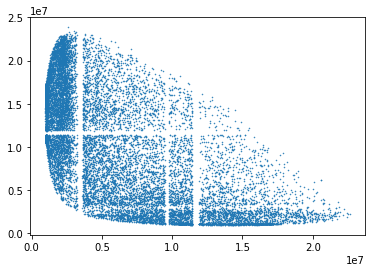
\includegraphics[width=0.8\textwidth]{plots/real_data_dalitz_removed_resonances.png}
  \caption{Dalitz Plot für echte Daten mit entsprechenden Schnitten auf die Massen der Zwischenresonanzen.}
  \label{fig:schnibbelDalitz}
\end{figure}

\subsection{Lokale CP-Verletzung}

In Abschnit \ref{sec:globCP} wurde die globale CP-Verletzung für simulierte Daten untersucht.
Nun soll zunächst die CP-Verletzung auf lokaler Ebene, also nur in einem gewissen Bereich von $M_{1,2}$ und $M_{1,3}$, für echte Daten untersucht werden.
Um die CP-Verletzung untersuchen zu können, werden zwei Dalitz Plots angefertigt, die nach der Ladung der Ausgangs-$B$-Mesonen aufgeteilt wurden.
Dies ist in Abbildung \ref{fig:plusDalitz} und \ref{fig:minusDalitz} zu sehen.

\begin{figure}
  \centering
  \minipage[c]{0.48\textwidth}%Minipage???
    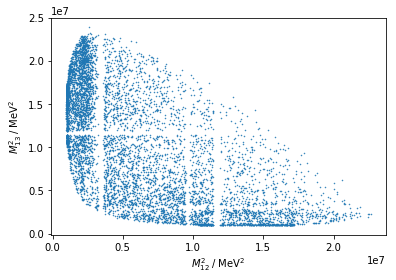
\includegraphics[width=\linewidth]{plots/real_data_dalitz_positive_B.png}
    \caption{Dalitz plot für $B^+$.
    \label{fig:plusDalitz}}
  \endminipage\hfill
  \minipage[c]{0.48\textwidth}
    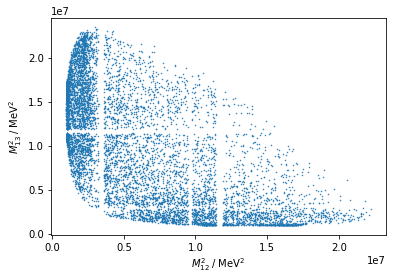
\includegraphics[width=\linewidth]{plots/real_data_negative_B.png}
    \caption{Dalitz plot für $B^-$.
    \label{fig:minusDalitz}}
  \endminipage
  \label{fig:split_resonances}
\end{figure}

Die Einträge in den Dalitz Plots werden histogrammiert.
So stehen in den entsprechenden Dalitz Plots in jedem Bin die Anzahl der entsprechenden $B^\pm$-Mesonen.
Daraus wird die CP-Verletzung in jedem Bin nach Gleichung \ref{eqn:globCP} berechnet.
Die Größe der CP-Verletzung in jedem Bin ist in Abbildung \ref{fig:locCP} zu sehen.

\begin{figure}
  \centering
  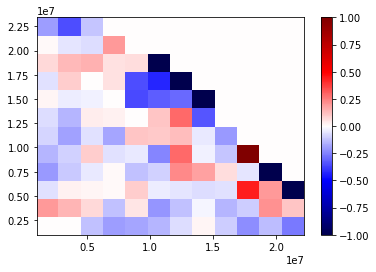
\includegraphics[width=0.8\textwidth]{plots/hist_asymmetrie_dalitz.png}
  \caption{Gebinnte CP-Verletzung berechnet aus den entsprechenden $B$-Mesonen aus dem gebinnten Dalitz Plot.}
  \label{fig:locCP}
\end{figure}

Allerdings bedeutet die Beobachtung einer großen Asymmetie in einer Region nicht unbedingt, dass dort auch wirklich CP-Verletzung beobachtbar ist.
Dafür muss sich in der entsprechenden Region eine gewisse Signifikanz zeigen.
Diese sollte für einen Hinweis größer als drei und für einen Beweis größer als fünf Standardabweichungen betragen.
Wird die Unsicherheit zu groß, so kann die Asymmetie auch kompatibel mit 0 sein, obwohl eine gewisse Asymmetie festgestellt werden konnte.
Die Unsicherheit wird analog zu Gleichung \ref{eqn:sigmaCP} berechnet und die Signifikanz analog zu Gleichung \ref{eqn:signifikanzCP}.
Diese gebinnte Unsicherheit ist in Abbildung \ref{fig:locSigma} zu sehen.
Daraus lässt sich die Signifikanz berechnen, die in Abbildung \ref{fig:locSigni} dargestellt ist.

\begin{figure}
  \begin{subfigure}{0.5\textwidth}
    \centering
    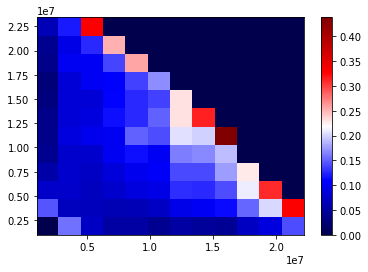
\includegraphics[width=\linewidth]{plots/real_data_uncertainty_asymmetrie_dalitz.png}
    \caption{Unsicherheit der berechneten Asymmetrie.}
    \label{fig:locSigma}
  \end{subfigure}%
  \begin{subfigure}{0.5\textwidth}
    \centering
    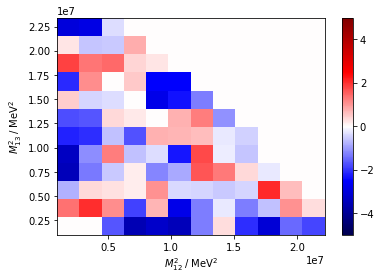
\includegraphics[width=\linewidth]{plots/real_data_significance_dalitz.png}
    \caption{Signifikanz der berechneten Asymmetrie.}
    \label{fig:locSigni}
  \end{subfigure}%
  \label{fig:sigundsig}
  \caption{Unsicherheit und Signifikanz der berechneten Asymmetrien.}
\end{figure}

Für die konkrete Untersuchung einer lokalen CP-Verletzung wird eine Region aus $M_{1,2}$ und $M_{1,3}$ herausgesucht, die eine Ansammlung von Bins aufweist, die eine gewisse Signifikanz besitzen.
Dieser Bereich wird auf $\SI{0}{\mega\electronvolt\squared} < M_{1,2} < \SI{5}{\mega\electronvolt\squared}$ und $\SI{5}{\mega\electronvolt\squared} < M_{1,2} < \SI{15}{\mega\electronvolt\squared}$ festgelegt.
Daher wird in der folgenden Untersuchung nur Ereignisse aus diesem Bereich berücksichtigt.
Die Asymmetrie berechnet sich dann in dem Bereich zu

% muss das nicht mega electronvolt^2 sein? da 0.5x10^7 ev^2 ja 5 MeV^2 sind

\begin{align*}
  A &= 0.052. \\%Hier steht gerade im Notebook nichts mehr zu
  \intertext{Die entsprechende Unsicherheit beträgt}
  \sigma_A &\approx 0.008 . \\
  \intertext{Dies entspricht somit einer Signifikanz von}
  \text{Signifikanz} &\approx 6.451 . \\
  \intertext{Allerdings muss die Produktionsasymmetrie berücksichtig werden. Die Signifikanz berechnet sich damit zu}
  \text{Signifikanz}_\text{sys} &\approx 4.071 .
\end{align*}

Mit dieser Signifikanz von $\text{Signifikanz}_\text{sys} \approx 4.071$ wurde somit ein guter Hinweis auf die lokale CP-Verletzung gefunden.
Dies wird durch die Abbildung \ref{fig:vglCP} unterstrichen.
Dort ist die Anzahl der $B$-Mesonen für beide Ladungen gegeneinander dargestellt.
Der Unterschied zwischen den beiden Ladungen ist auch hier noch einmal deutlich zu sehen.

\begin{figure}
  \centering
  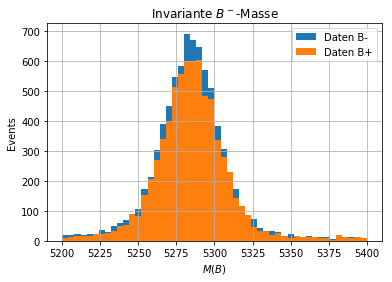
\includegraphics[width=0.8\textwidth]{plots/real_data_local_region_inv_mass_B.png}
  \caption{Vergleich der Anzahl an $B$-Mesonen der beiden Ladungen in dem untersuchten Bereich von $M_{1,2}$ und $M_{1,3}$. Der Unterschied zwischen den Ladungen ist deutlich sichtbar.}
  \label{fig:vglCP}
\end{figure}




.
